
\section{Autenticare le richieste: la scelta del servizio e la sua integrazione}


Poiché la modalità di autenticazione rappresenta
un elemento importante per l'esperienza utente,
in quanto deve assicurare un accesso sicuro all'applicazione mantenendone la semplicità,
la facilità del processo di autenticazione è imperativa.
L'applicazione deve consentire la possibilità di registrarsi
creando un nuovo account dedicato,
ma è altrettanto essenziale che permetta agli utenti di farlo anche
tramite il proprio servizio di autenticazione preferito,
migliorando sensibilmente l'usabilità e l'apprezzamento.
Di conseguenza, il sistema di gestione degli accessi deve 
sia supportare la registrazione e la gestione autonoma 
degli account specifici per il servizio,
sia fornire l'integrazione con provider di autenticazione esterni.\\
\\
Per lo scopo, Azure fornisce Microsoft Entra ID,
che fa parte della suite di servizi di autenticazione e autorizzazione, Microsoft Entra.
Sebbene sia teoricamente in grado di soddisfare i requisiti sopra indicati,
la complessità della documentazione e le difficoltà
riscontrate nell'integrazione con il servizio dell'applicativo
hanno portato a valutare soluzioni alternative negli ambienti cloud.\\
\\
\begin{wrapfigure}{o}{0.25\textwidth}
    \centering
    
\includegraphics[height=.12\textheight]{firebase.png}
    Firebase Authentication
\end{wrapfigure}
La scelta è ricaduta su Firebase Authentication,
il servizio di autenticazione fornito da Google Cloud Provider,
che garantisce sia la possibilità di creare account dedicati
che di collegarsi attraverso altri servizi di autenticazione.
Presenta librerie di integrazione sia tramite Flutter
che tramite C\# che risultano facili da utilizzare,
oltre a fornire una piattaforma di gestione con un'interfaccia chiara e intuitiva.
Dal punto di vista economico, il servizio risulta vantaggioso,
essendo gratuito fino ai cinquantamila utenti mensili attivi.\\
\clearpage
Firebase si integra facilmente con Flutter,
fornendo una libreria che gestisce completamente 
l'ottenimento e il mantenimento dei token di autenticazione,
a partire dalle credenziali o dalle verifiche precedenti.
Per ogni richiesta del client che richiede identificazione
il servizio apposito intercetta il messaggio,
recupera il token ottenuto durante la fase di login e glielo allega.
Alla ricezione del messaggio, il server estrae il token dalla richiesta,
per poi contattare Firebase grazie all'astrazione fornita dalla libreria.
Firebase controlla il token e, se corretto,
ne restituisce i dati dell'account relativo.\\
\begin{figure}[htpb]
    \centering
    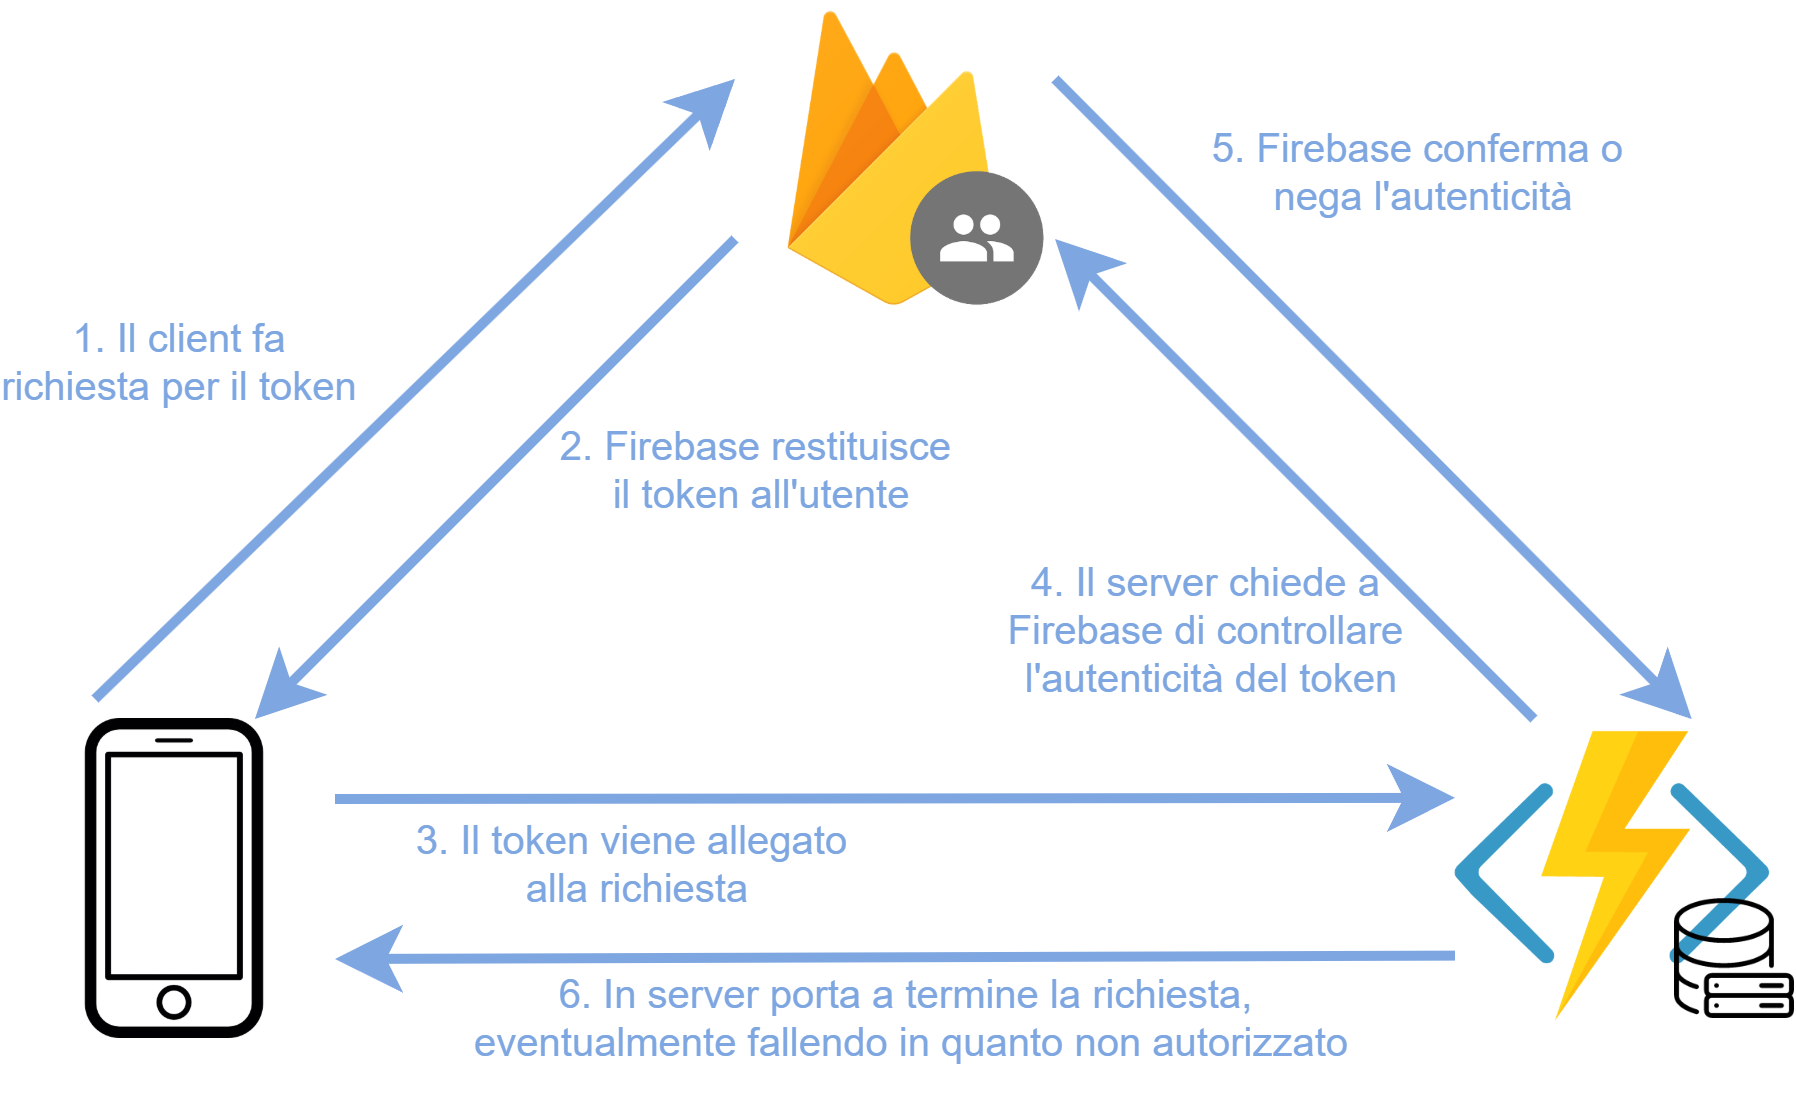
\includegraphics[width=\textwidth]{TokenLogin.png}
    \caption{Fasi di ottenimento e uso del token}
\end{figure}

Uno dei requisiti del progetto prevede
che ogni account sia associato in modo univoco a un singolo utente.
Durante la fase di registrazione, tuttavia,
l'account viene inizialmente registrato nel database gestito da Firebase.
Pertanto, al primo accesso, il server, dopo aver verificato l'autenticità della richiesta,
provvede a creare una copia dell'account,
generando poi il relativo nuovo oggetto utente e il primo profilo associato.\\
\\
\begin{figure}[htpb]
    \centering
    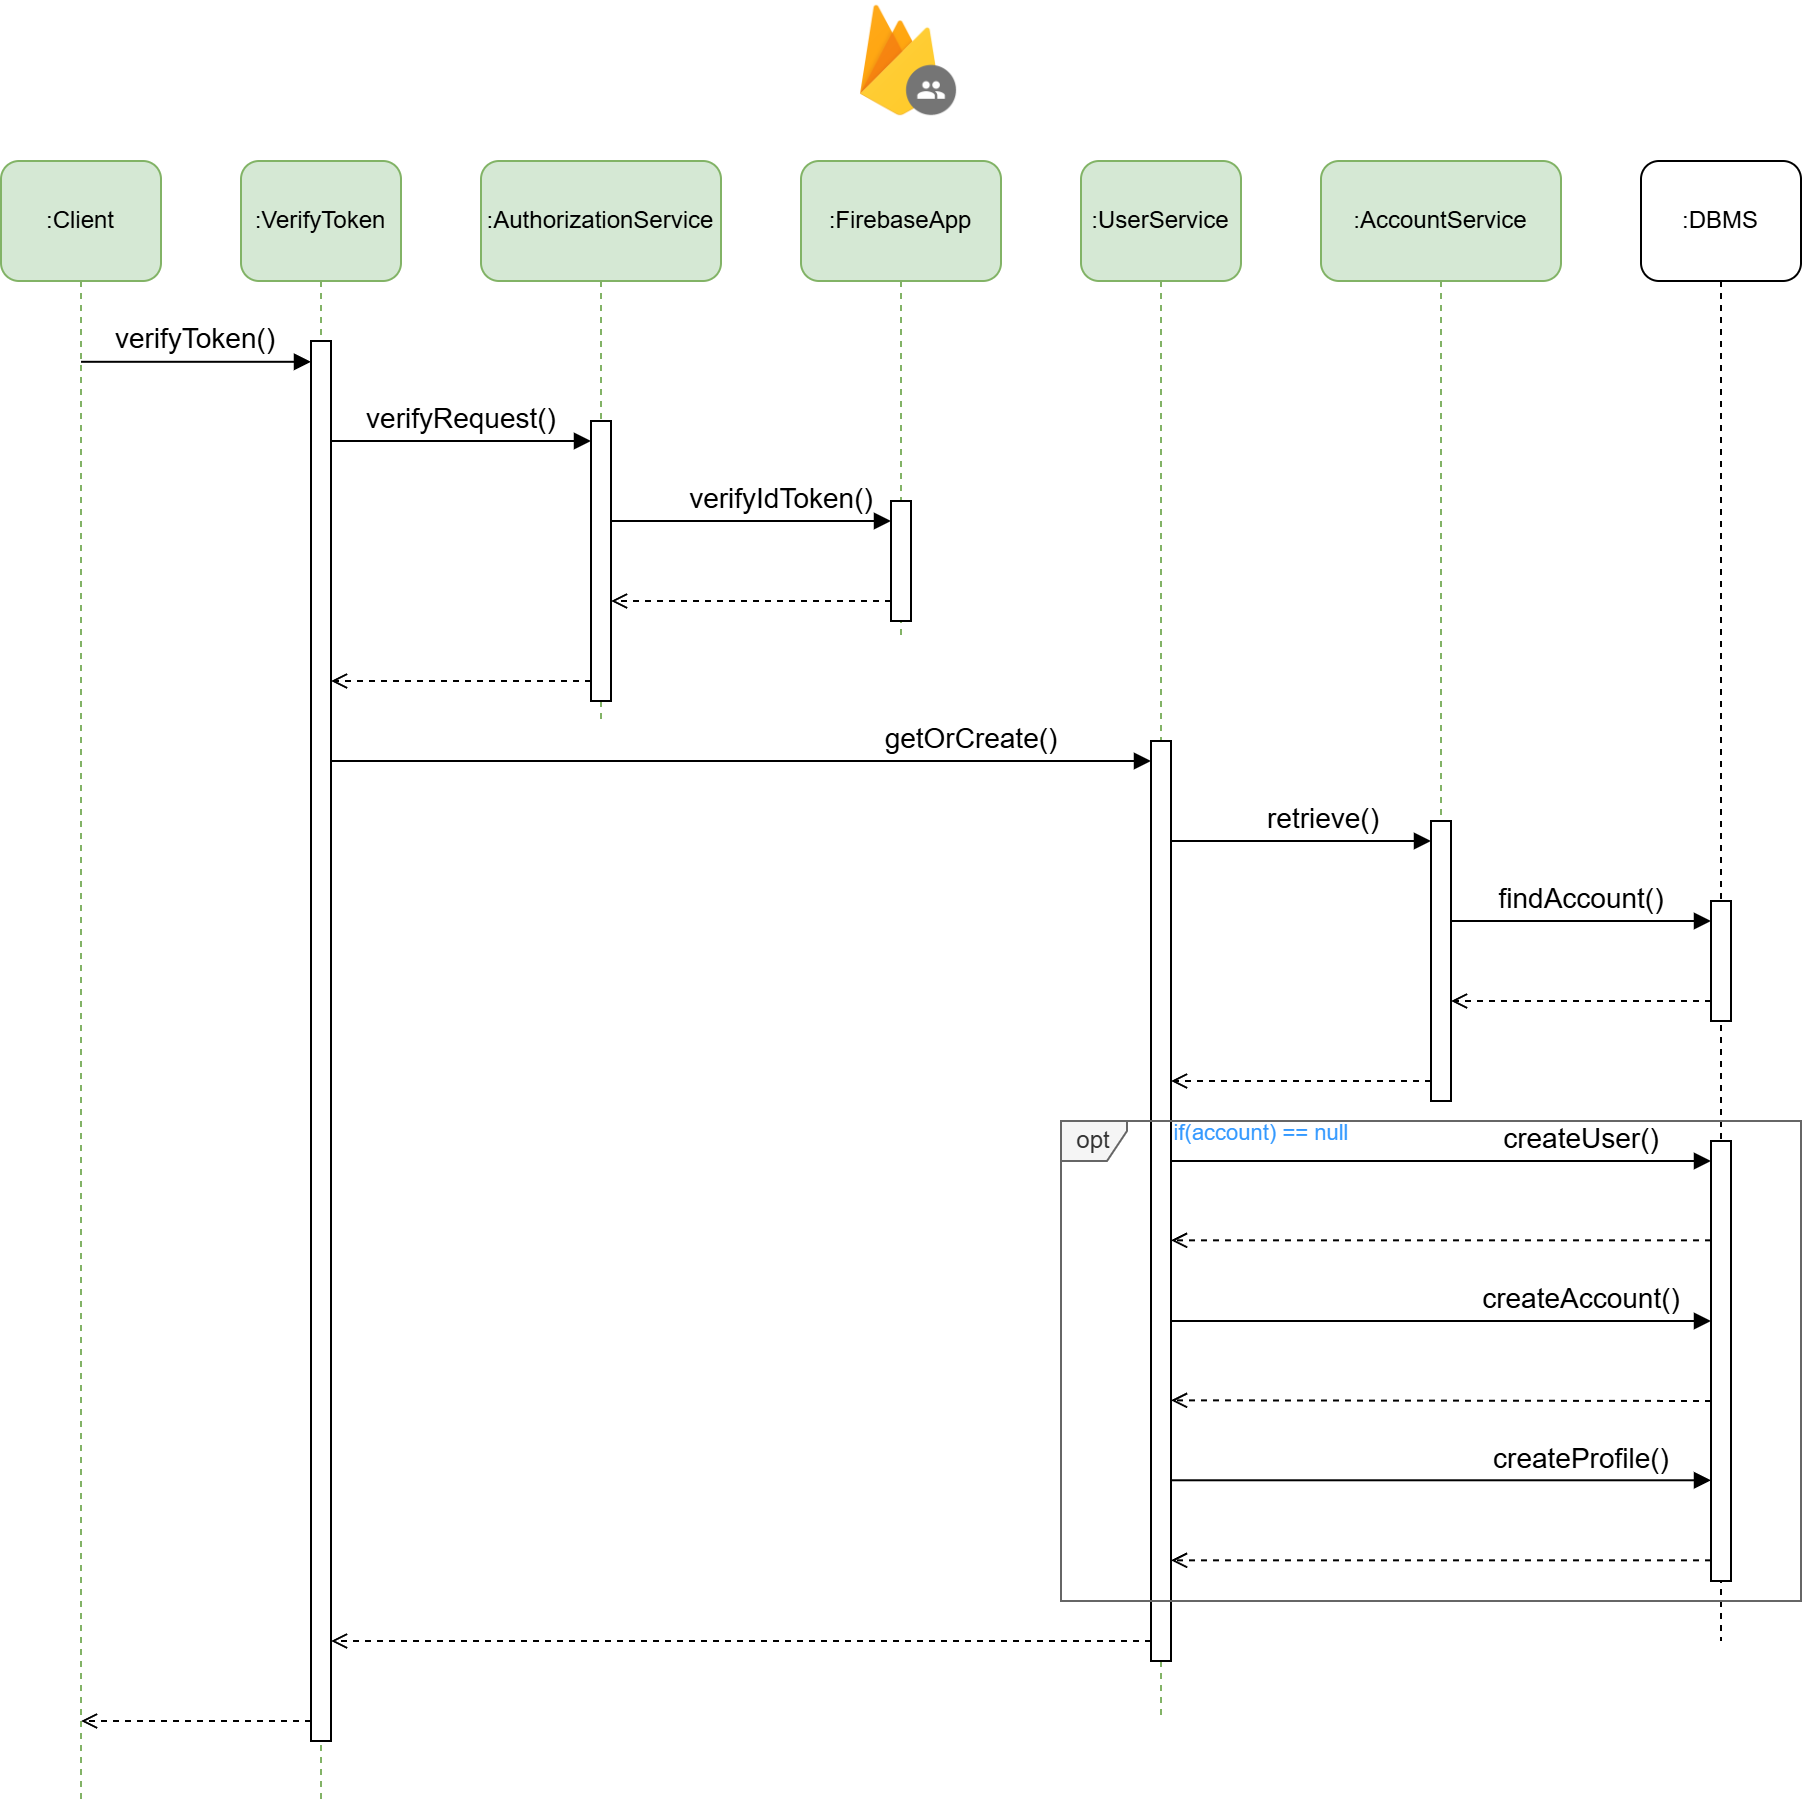
\includegraphics[width=\textwidth]{IIVerifyToken2.png}
    \caption{Diagramma di sequenza per la creazione di un account}
\end{figure}

\clearpage
\section{Uno sguardo sulla sicurezza: segreti e protocolli}
\begin{wrapfigure}{o}{0.25\textwidth}
    \centering
    
\includegraphics[height=.12\textheight]{keyvault.png}
    Azure Key Vault
\end{wrapfigure}
Il collegamento tra i vari componenti all'interno dell'ambiente Azure
richiede l'utilizzo di chiavi e stringhe di connessione.
Il salvataggio di tutte le chiavi è stato affidato al servizio Azure Key Vault,
un server che permette la centralizzazione dei dati sensibili,
cifrando il contenuto e garantendo un maggiore controllo sul loro utilizzo.\\
I servizi, in particolare le Azure Functions,
contatteranno quando necessario il Key Vault per l'ottenimento delle chiavi necessarie,
di fatto separando la logica implementativa dai segreti necessari per la sua esecuzione,
riducendo così il rischio di una perdita delle chiavi derivata da un errore dello sviluppo.\\
\\
Le comunicazioni tra i vari componenti devono avvenire in sicurezza,
garantendo autenticità e confidenzialità.
Per questo motivo tutte le comunicazioni tra dispositivi client e
i vari servizi utilizzano la tecnologia TLS,
che permette di cifrare i messaggi grazie a uno standard collaudato.
In particolare, le comunicazioni tra i client e Azure Functions,
così come con Firebase Authentication e il server per la persistenza delle immagini,
avvengono tramite protocollo HTTPS,
mentre le comunicazioni con il server per gli aggiornamenti in tempo reale usano il protocollo WSS.\\
\\
Il rischio di saturazione delle risorse viene mitigato
aggiungendo un duplice controllo sulle dimensioni delle richieste.
In primo luogo si limita la dimensione massima della singola richiesta,
facendo particolare attenzione alle richieste che contengono immagini,
controllandola sia nel momento dell'invio che nel momento della ricezione.
Inoltre, alla fine di ogni richiesta più grande di una determinata soglia,
la dimensione viene sommata alle precedenti nell'ultimo periodo e,
se la somma risulta troppo elevata, viene limitato l'utilizzo per quell'utente.\\
\\
Per evitare un numero eccessivo di richieste totali,
che possono provocare anch'esse una riduzione del servizio,
è possibile integrare nel sistema risorse create appositamente da Azure,
quali Azure DDOS Protection.\\
\\
L'accesso al database è ristretto alle sole risorse Azure,
garantendo l'isolamento dall'esterno,
che comprometterebbe altrimenti l'affidabilità dei dati.\\
\\
Infine, è bene che gli identificativi delle entità del dominio 
siano composti da codici hash univoci, 
permettendo l'identificazione dell'oggetto ma senza senza rivelare ulteriori informazioni.
In particolare, il recupero delle immagini
avviene grazie a un link univoco formato dalla combinazione
degli identificativi dell'evento e dell'immagine.
L'immagine risulta pubblicamente accessibile a chiunque abbia il link corretto.
Utilizzando i codici di hash diventa molto complicato ritrovare le immagini
senza essere a conoscenza di entrambi gli identificativi,
che non avendo natura incrementale ma randomicamente distribuita rende
indovinare l'unica strategia per trovare un link valido.

\section{Monitoraggio dei servizi}

Il monitoraggio del sistema è attuato in due modalità:
tramite il salvataggio dei log e grazie al controllo delle prestazioni del sistema.\\
\\
Relativamente a Firebase Authentication sono fornite, incluse nel servizio,
sia le interfacce per il controllo delle prestazioni che per la gestione dei log.
Non è quindi richiesta alcuna ulteriore azione.\\
\begin{wrapfigure}{o}{0.25\textwidth}
    \centering
    
\includegraphics[height=.12\textheight]{insights.png}
    Azure Application Insights
\end{wrapfigure}
Per monitorare le Azure Functions sarà invece necessario
affiancargli un'istanza di Azure Application Insights,
servizio nato appositamente per controllare il funzionamento e la risposta dei servizi Azure.
Una volta collegato il servizioApplication Insight
permette la presentazione e l'analisi di numerose metriche,
quali il tempo medio di risposta e il consumo di risorse.
Consente inoltre di testare la risposta dell'applicativo
simulando diversi scenari e riassumendo il loro comportamento.\\
\\
La creazione dei log è invece delegata al programmatore,
in quanto è necessario integrarli nel codice.
Nel momento della creazione, ogni funzione riceve, tramite dependency injection,
un servizio Logger che permette la creazione e il salvataggio dei log.
La funzione non dovrà fare altro che chiamare
il metodo apposito per generare e salvare un log.
Tali log saranno poi consultabili e analizzabili tramite l'interfaccia fornita da Azure Application Insight.
\clearpage